\chapter{Analysis Techniques}\label{ch:analysis}

\section{Mathematical Tools}

Before going into analysis techniques of the FD schemes presented in this chapter, some mathematical tools used for these techniques will be presented. 


\subsubsection{Continuous time}
For two functions $f(x)$ and $g(x)$ and $x\in\D$ their $l_2$ inner product along with the $l_2$ norm is defined as
\begin{equation}\label{eq:contInnerProd}
    \langle f, g\rangle_\D = \int_\D fg dx \quad \text{and} \quad \lVert f \rVert_\D = \sqrt{\langle f, f \rangle_\D}
\end{equation}

\subsubsection{Integration by parts}


\subsubsection{Discrete-time}
Inner product of any time series $f^n$ and $g^n$ and the discrete counterpart to \eqref{eq:contInnerProd} is
\begin{equation}\label{eq:discInnerProd}
    \langle f^n, g^n \rangle_\D = \sum_{l\in\D} h f_l^n g_l^n
\end{equation}
where the multiplication by $h$ is the discrete counterpart of $dx$ the continuous definition. 


\subsection{Matrices}
For several purposes, such as implementation in MATLAB and several analysis techniques described shortly, is useful to write an FD scheme in \textit{matrix form}. 

In this document, matrices and vectors are written using bold symbols. \SWcomment[Many notations exist, blabla $\bar a$ $\vec a$] A matrix uses a capital letter whereas vectors are decapitalised. The dimensions of a matrix are denoted using ``$row \times column$''. A $6\times 14$ matrix, for example, thus has $6$ rows and $14$ columns. Along those lines, a \textit{row vector} is a matrix with $1$ row and more than $1$ column and a \textit{column vector} is a matrix with $1$ column and more than $1$ row. \SWcomment[If a matrix has only $1$ row and $1$ column, it can be used as a \textit{scalar}.]

\subsubsection{Matrix Multiplication}
In order for matrix multiplication (including matrix-vector multiplication) to be valid, the number of columns of the first matrix needs to be equal to the number of rows in the second matrix. The result will then be a matrix with a number of rows equal to that of the first matrix and a number of columns equal to that of the second matrix. See Figure \ref{fig:matrixVector} for reference.

As an example, consider the $L
\times M$ matrix $
\A$ and a $M\times N$ matrix $
\B$. The multiplication $\A\B$ is defined as the number of columns of matrix $
\A$ ($M$) is equal to the number of rows of matrix $\B$ (also $M$). The result, $\C$, is a $L \times N$ matrix. The multiplication $\B\A$ is undefined as the number of columns of the first matrix does not match the number of rows in the second matrix. 

Multiplying two matrices written in their dimensions as 
\begin{equation}
    \overbrace{(L\times M)}^{\A}\cdot \overbrace{(M\times N)}^{\B} = \overbrace{(L
    \times N)}^{\C}
\end{equation}
 
\begin{figure}[h]
    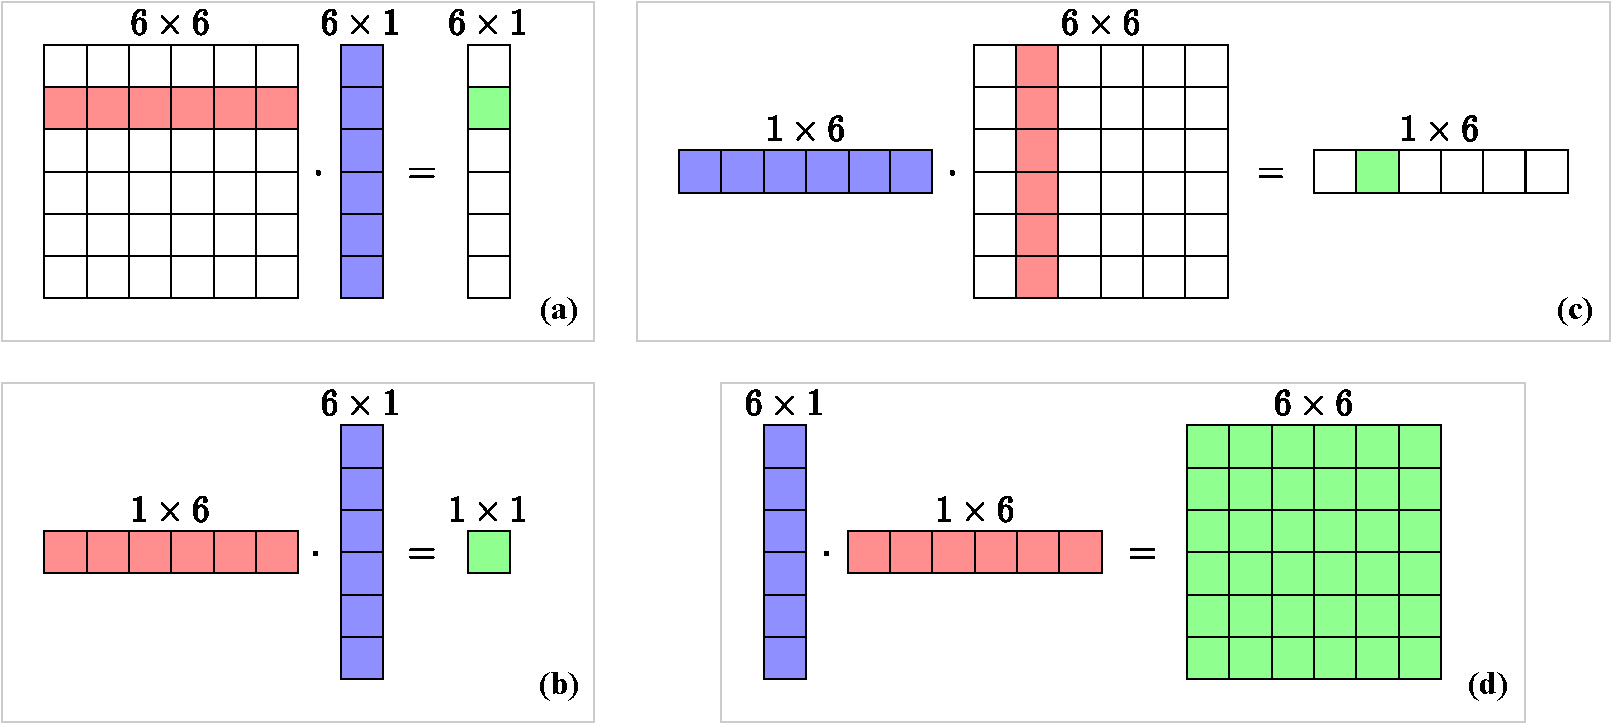
\includegraphics[width=\textwidth]{figures/fdtd/matrixVector2.pdf}
    \caption{Visualisation of valid matrix(-vector) multiplications. \label{fig:matrixVector}}
\end{figure}

\subsubsection{In a FDTD context}
Matrix multiplication when working with FDTD methods usually involves multiplying a square matrix (with equal rows and columns) onto a column vector (see Figure \ref{fig:matrixVector}a). Consider a square matrix with $(N+1)\times (N+1)$ elements $\A$ and a $(N+1) \times 1$ column vector $\u$. Multiplying these results in a $(N+1) \times 1$ column vector $\w$:
\begin{equation}
    \A\u = \w.
\end{equation}
Expanding this operation results in 
\begin{equation}
    \underbrace{\begin{bmatrix}
        a_{00} & a_{01} & \hdots & a_{0N}\\
        a_{10} & a_{11} & \hdots & a_{2N}\\
        \vdots & \vdots & &\vdots\\
        a_{N0} & a_{N1} & \hdots & a_{NN}
    \end{bmatrix}}_{\A}
    \underbrace{\begin{bmatrix}
        u_0\\
        u_1\\
        \vdots\\
        u_N
    \end{bmatrix}}_{\u} = 
    \underbrace{\begin{bmatrix}
        a_{00}u_0 + a_{01}u_1 + \hdots + a_{0N}u_N\\
        a_{10}u_0 + a_{11}u_1 + \hdots + a_{1N}u_N\\
        \vdots\\
        a_{N0}u_0 + a_{N1}u_1 + \hdots + a_{NN}u_N
    \end{bmatrix}}_{\w}
\end{equation}


\subsubsection{Operators in Matrix Form}
The FD operators approximating first-order spatial derivatives in \eqref{eq:discFirstSpace} can be written in matrix form according to
\begin{gather*}\small
    \mathbf{D}_{x+} = \frac{1}{h}\begin{bmatrix}
        \ddots &\ddots & & & \mathbf{0}&\\
         & -1 & 1 & & & \\
        & & -1 & 1 & & \\
        & & & -1 & 1 & \\
        & & & & -1 & \ddots\\
        &\mathbf{0} & & & & \ddots \\
    \end{bmatrix}
    \quad
    \mathbf{D}_{x-} = \frac{1}{h}\begin{bmatrix}
        \ddots & & & & \mathbf{0}&\\
        \ddots & 1 & & & & \\
        & -1 & 1 & & & \\
        & & -1 & 1 & & \\
        & & & -1 & 1 & \\
        &\mathbf{0} & & & \ddots & \ddots \\
    \end{bmatrix}\\
    \\
    \mathbf{D}_{x\cdot} = \frac{1}{2h}\begin{bmatrix}\small
        \ddots &\ddots & & & \mathbf{0}&\\
        \ddots & 0 & 1 & & & \\
        & -1 & 0 & 1 & & \\
        & & -1 & 0 & 1 & \\
        & & & -1 & 0 & \ddots \\
        &\mathbf{0} & & & \ddots & \ddots \\
    \end{bmatrix}\\
\end{gather*}
The matrices $\mathbf{D}_{x+}$ and $\mathbf{D}_{x-}$ can be multiplied to get $\Dxx$:
\begin{equation}\small
    \Dxx = \mathbf{D}_{x+}\mathbf{D}_{x-} = \frac{1}{h^2}\begin{bmatrix}
        \ddots &\ddots & & & \mathbf{0}&\\
        \ddots & -2 & 1 & & & \\
        & 1 & -2 & 1 & & \\
        & & 1 & -2 & 1 & \\
        & & & 1 & -2 & \ddots \\
        &\mathbf{0} & & & \ddots & \ddots \\
    \end{bmatrix}.
\end{equation}
%
Averaging operators $\mxp$, $\mxm$ and $\mxd$ are defined in a similar way:

\begin{gather*}
    \mathbf{M}_{x+} = \frac{1}{2}\begin{bmatrix}
        \ddots &\ddots & & & \mathbf{0}&\\
         & 1 & 1 & & & \\
        & & 1 & 1 & & \\
        & & & 1 & 1 & \\
        & & & & 1 & \ddots\\
        &\mathbf{0} & & & & \ddots \\
    \end{bmatrix}
    \qquad
    \mathbf{M}_{x-} = \frac{1}{2}\begin{bmatrix}
        \ddots & & & & \mathbf{0}&\\
        \ddots & 1 & & & & \\
        & 1 & 1 & & & \\
        & & 1 & 1 & & \\
        & & & 1 & 1 & \\
        &\mathbf{0} & & & \ddots & \ddots \\
    \end{bmatrix}\\
    \\
    \mathbf{M}_{x\cdot} = \frac{1}{2}\begin{bmatrix}
        \ddots &\ddots & & & \mathbf{0}&\\
        \ddots & 0 & 1 & & & \\
        & 1 & 0 & 1 & & \\
        & & 1 & 0 & 1 & \\
        & & & 1 & 0 & \ddots \\
        &\mathbf{0} & & & \ddots & \ddots \\
    \end{bmatrix}\\
\end{gather*}

It is important to notice that only spatial operators are written in this matrix form and then applied to state vectors at different time steps ($n+1$, $n$ and $n-1$). 

Finally, the identity matrix is a matrix with only $1$s on the diagonal and $0$s elsewhere as
\begin{equation}
    \I = \begin{bmatrix}
        \ddots & & & & \mathbf{0}&\\
         & 1 & & & & \\
        & & 1 & & & \\
        & & & 1 & & \\
        & & & & 1 & \\
        &\mathbf{0} & & &  & \ddots \\
    \end{bmatrix}\\
\end{equation}
\subsubsection{Schemes and Update Equations in Matrix Form}
With these building blocks we can write Eq. \eqref{eq:1DwaveFDS} in matrix form. The values of the grid function $\uln$ can be stored in a state vector according to $\u^n = [u_0^n, u_1^n, \hdots, u_N^n]^T$ where $T$ denotes the transpose operation. The FD scheme in \eqref{eq:1DwaveFDS} can then be written in matrix form as
\begin{equation}\label{eq:1DwaveMatrix}
    \frac{1}{k^2}\left(\u^{n+1} - 2 \u + \u^{n-1}\right) = c^2 \Dxx \u^n,
\end{equation}
and rewritten to a matrix form of the update equation
\begin{equation}
    \u^{n+1} = (2\I + c^2k^2 \Dxx )\u^n - \u^{n-1}.
\end{equation}
The identity matrix is necessary here for correct matrix addition.

\subsection{System of Linear Equations}
A number of unknowns described by the same number of equations can be solved using a 

\section{von Neumann Analysis}\label{sec:stabilityAnalysis}
Much literature gives the stability condition using an ``it can be shown that'' argument (fx. \cite{Bilbao2009}). Here, I would like to take the opportunity to 

Finding stability conditions for models

Sin identity:
\begin{equation}\label{eq:sinIdentity}
    \sin(x) = \frac{e^{jx} - e^{-jx}}{2j}\ \ \Rightarrow \ \ \sin^2(x) %= \frac{e^{j2x} - 2e^{jx-jx}+ e^{-j2x}}{-4} 
    = \frac{e^{j2x} + e^{-j2x}}{-4} + \frac{1}{2}.
\end{equation}
Cos identity:
\begin{equation}\label{eq:cosIdentity}
    \cos(x) = \frac{e^{jx} + e^{-jx}}{2}\ \ \Rightarrow \ \ \cos^2(x) %= \frac{e^{j2x} + 2e^{jx-jx}+ e^{-j2x}}{4} 
    = \frac{e^{j2x} + e^{-j2x}}{4} + \frac{1}{2}.
\end{equation}

One can analyse a \todo{check `a' or `an' FD scheme}FD scheme by 
\begin{equation}
    u_l^n = z^n e^{jl\beta h}
\end{equation}
where $\beta$ is a real wavenumber. Important to remember is that without a shift in space (fx. $l+1$) or time (fx. $n-1$) $l = 0$ or $n=0$ respectively:
\begin{subequations} \label{eq:identitiesZ}
    \begin{align}
        u_l^n &= z^0 e^{j0\beta h} = 1\\
        u_{l+1}^n &= z^0 e^{j1\beta h} = e^{j\beta h}\\
        u_{l-1}^n &= z^0 e^{j(-1)\beta h} = e^{-j\beta h}\\
        u_{l+2}^n &= z^0 e^{j2\beta h} = e^{j\beta h}\\
        u_{l-2}^n &= z^0 e^{j(-2)\beta h}= e^{-j2\beta h}\\
        u_l^{n+1}&= z^1 e^{j0\beta h} = z\\
        u_l^{n-1}&= z^{-1} e^{j0\beta h} = z^{-1}
    \end{align}
\end{subequations}

\todo{Talk about solution of }

\section{Energy Analysis}\label{sec:energyAnalysis}

The Hamiltonian or $\mathfrak{H}$

Multiplying scheme by $\left(\dtd \uln \right)$

Debugging physical models...
One can plot the energy of the system and in a lossless system, the rate of change of the total energy should be 0, i.e.,
\begin{equation}\label{eq:unchangedEnergy}
    \delta_{t+}\mathfrak{h} = 0 \quad \Longrightarrow \quad \mathfrak{h}^n = \mathfrak{h}^0.
\end{equation}
.

Although the energy of a lossless system should be unchanged according to Eq. \eqref{eq:unchangedEnergy}, but in a finite precision simulation, ultra slight fluctuations of the energy should be visible due to rounding errors. 

Plotting energy should be within \textit{machine precision}, which mostly is in the range of $10^{-15}$

\subsubsection{Product Identities}
Some useful identities used in this work are
\begin{subequations}
    \begin{align}
        (\dtd \uln)(\dtt \uln) &= \dtp \left(\frac{1}{2}(\dtm \uln)^2\right),\label{eq:prodIdentity1}\\
        (\dtd \uln)\uln &= \dtp \left(\frac{1}{2}\uln e_{t-}\uln\right),\label{eq:prodIdentity2}\\
        (\dtp \uln)(\mtp \uln) &= \dtp \left(\frac{1}{2}(\uln)^2\right),\label{eq:prodIdentity3}\\
        (\dtd \uln)(\mu_{t\cdot}\uln) &= \dtd\left(\frac{1}{2} (\uln)^2\right).\label{eq:prodIdentity4}
    \end{align}
\end{subequations}
Again, these can be used for spatial derivatives as well by substituting the `$t$' subscripts for `$x$'. Also  to 

When an operator is applied to a product of two grid functions, the discrete counter part of the product rule needs to be used according to
\begin{equation}
    \dtp (\uln\wln) = (\dtp \uln)(\mtp\wln) + (\mtp \uln)(\dtp \wln).
\end{equation}


\subsection{Stability Analysis}
One can perform stability analysis using the energy analysis techniques presented here. To arrive at a condition the energy must be \textit{positive definite} 

\section{Modal Analysis}
\label{sec:modalAnalysis}
Modes are the resonant frequencies of a system. The amout of modes that a discrete system contains dependends on the amount of moving points. A mass-spring system thus has one resonating mode, but a FD scheme of the 1D wave equation with $N = 30$ and Dirichlet boundary conditions will have $29$ modes. This section will show how to obtain the modes of an FD scheme implementing the 1D wave equation. 

We start by using the the matrix form of FD scheme \eqref{eq:1DwaveFDS} from Eq. \eqref{eq:1DwaveMatrix}
\begin{equation*}
    \frac{1}{k^2}\left(\u^{n+1}-2\u^n+\u^{n-1}\right) = c^2 \Dxx\u.
\end{equation*}
Following \cite{theBible} we assume a solution of the form $\u = \boldsymbol{\phi}z^n$ \todo{more explanation}. Substituting this into Eq. \eqref{eq:matrixForm1D} yields the characteristic equation
\begin{equation}
    (z - 2 + z^{-1})\boldsymbol{\phi} = c^2k^2\Dxx \boldsymbol{\phi}.
\end{equation}
This is an eigenvalue problem where the $p$'th solution is defined as 
\begin{gather}
    z_p-2+z_p^{-1} = c^2k^2\text{eig}_p(\Dxx)\nonumber\\
    z_p+(-2-c^2k^2\text{eig}_p(\Dxx))+z_p^{-1}=0
\end{gather}
where $\text{eig}_p(\cdot)$ denoting the $p$th eigenvalue of `$\cdot$'. \SWcomment[If the CFL condition for the scheme is satisfied, the roots will lie on the unit circle.] Furthermore we can substitute a test solution $z_p=e^{j\omega_pk}$ solve for the eigenfrequencies:
\begin{align*}
    e^{j\omega_pk}+e^{-j\omega_pk}-2-c^2k^2\text{eig}_p(\Dxx)&=0\\
    \frac{e^{j\omega_pk}+e^{-j\omega_pk}}{-4}+\frac{1}{2}+\frac{c^2k^2}{4}\text{eig}_p(\Dxx)&=0
\end{align*}
Then using Eq. \eqref{eq:sinIdentity} we get
\begin{align}
    \sin^2(\omega_pk/2)+c^2k^2\text{eig}_p(\Dxx)&=0\nonumber\\
    \sin(\omega_pk/2)&=c k\sqrt{-\text{eig}_p(\Dxx)}\nonumber\\
    \omega_p &= \frac{2}{k}\sin^{-1}\left(c k\sqrt{-\text{eig}_p(\Dxx)}\right)
\end{align}
which is Eq. (6.53) in \cite{theBible}.

\section{Dispersion analysis}\label{sec:dispersionAnalysis}
